\section{Methods} \label{sec:methods}

In this section, we detail the methodology for benchmark and validation experiments used to assess the performance of the proposed shortcut-enabled reconstruction algorithm empirically.

\subsection{Generation of Benchmark Data}

For our benchmark experiments, we needed a sample of large-scale genomes to draw from to perform reconstructions on.
For this purpose, we performed simulations using the Cerebras CS-2
Wafer-Scale Engine, a recently introduced 850,000 core hardware accelerator device \citep{lie2023cerebras}.
Processor elements (PEs) in this architecture are arranged in a grid lattice where each processor is able to execute independently and communicate with neighboring PEs through message-passing, with tight per-core limitations on available memory.

To conduct these simulations, we used an extension of the island-model genetic algorithm framework presented in \citep{moreno2024trackable}.
This framework organizes simulated organisms into independent subpopulations hosted on each PE.
Synchronous tournament selection of size 2 is applied within each PE, and between generations agents are migrated between PEs asynchronously.

%The purpose of this simulation was to generate large-scale data using a simple model that can be explicitly manipulated to explore evolutionary regimes differing substantially in the depth of shared ancestry between organisms (known as phylogenetic richness).

A simple genome model was used, wherein agents were comprised of a single floating point value representing fitness.
Reproduction occurred asexually, with this value subject to normally-distributed mutation with 30\% probability.
(In the case of the purifying-regime treatment, the negative absolute value of a sampled mutation delta was applied.)
In tournament competitions to select parents for the subsequent generation, the parent was selected according to the higher fitness value with 10\% probability and was otherwise selected randomly.

To generate data representative of different evolutionary conditions, two treatments were applied:
\textbf{adaptive regime} and \textbf{purifying regime}.
Under the adaptive regime, mutations increasing fitness were allowed, introducing the possibility of selective sweeps.
By contrast, the purifying regime treatment allowed only the possibility of deleterious mutations
Previous work with this system demonstrated the purifying regime to exhibit substantially greater phylogenetic richness -- in line with expectation.

Fossil data were sampled on a rolling basis using asynchronous \texttt{memcpy} operations, where a representative agent was copied from device to host from each processor element on a rolling basis.
% https://github.com/mmore500/wse-async-ga/blob/31034c3b1f8127763807992916f20d7d3ea62919/slurm/2024-12-25/2024-12-25%2Blex12-async-ga.sh
The simulation was run for 5 million generation cycles.
A per-PE population size of 256 organisms was used, providing a net population size of 190.8 million organisms.
% https://osf.io/btg23 and https://osf.io/2my97
Over the course of the simulation, fossil genome collection of 1,999 (purifying regime) and 2,014 (adaptive regime) memcopy cycles elapsed.
% https://osf.io/btg23 and https://osf.io/2my97
Real-time runtime for each was 24 minutes.
For full details on the Wafer-Scale Engine, see \citep{moreno2024trackable}.

We used hstrat annotations comprising 64 single-bit markers, managed at runtime using a \texttt{tilted} curation policy, which favors dense retention of more recent marker data.

\subsection{Microbenchmark Experiments}

From this simulation (in both purifying and adaptive versions), we took a random sample of 10 million tips that could be used on a personal computer for various benchmarks, which were intended to test reconstruction performance.
First, we wanted to determine the asymptotic complexity of our new algorithm; to do this, we ran sub-samples of various sizes through the reconstruction pipeline and measured the time it took in the reconstruction step.
This was done for both adaptive and purifying simulations in order to test different arrangements of data.

We then wanted to compare the performance of this algorithm with the previous naive trie algorithm.
We did this by again taking subsamples of the 10 million tips and running both algorithms on the subsample and timing how long it took to process all the tips.
Given that the naive algorithm is significantly slower, our subsample sizes were limited to up to 10,000 tips.

Because of this, we also wanted to determine the performance of the search table algorithm on larger data, and more importantly, determine the asymptotic complexity of the approach. 
To do this, we performed runs of a 10 million tip reconstruction, where the time taken to insert each batch of 100 thousand tips was measured.
This way, we could determine if this time increases for later batches (i.e. larger trees), or stays about constant.
We also performed this process on both adaptive and purifying regimes, so that we could determine if there were potential differences depending on the evolutionary scheme.
Another test we did to more directly measure complexity was taking a range of sub-samples from the original sample up to 10 million tips, ran the end-to-end pipeline, and measured the time taken on the reconstruction step alone.

These examples were all run on a 2019 MacBook Pro (2.3GHz 8-Core Intel i9, 16GB RAM) using a benchmark script attached with our supplemental material \citep{supplemental}.

\subsection{Macrobenchmark Experiments}

To assess the performance of our approach on large-scale workloads under real-world conditions, we supplemented microbenchmarks focusing on core trie extension and consolidation operations with two macrobenchmark trials comprising the full end-to-end reconstruction pipeline described in Section \ref{sec:pipeline}.
As mentioned in the figure, to save memory, we include a step that collapses unnecessary unifurcations (a parent having a single child, which is redundant information) -- for more details, see the supplemental \citep{supplemental}.
These end-to-end experiments used the \texttt{hstrat.dataframe.surface\_build\_tree} CLI module incorporated in the \texttt{hstrat} library.

These experiments were conducted using the full billion-element corpus of sampled genomes from Wafer-Scale Engine simulations.
We performed two trial reconstructions: one using genome data from the adaptive regime treatment and another under the purifying regime treatment.

Reconstructions were conducted on 100-core cluster node allocations.
% purifying log: https://osf.io/gj52m
Purifying-regime reconstruction was performed on an AMD EPYC 7763 Processor (2.445 GHz) with 128 cores and 2005 GB of memory.
% purifying log: https://osf.io/s3rzj
Adaptive-regime reconstruction was performed on an AMD EPYC 7H12 Processor (2.595 GHz) with 128 cores and 2005 GB of memory.
End-to-end experiments used the \texttt{hstrat.dataframe.surface\_build\_tree} CLI module incorporated in the \texttt{hstrat} library.

\subsection{Validation Tests}

One part of our algorithm that we aim to show is that it is essentially equivalent to the naive trie algorithm already implemented.
We assert that any decisions it makes could be made by the naive trie algorithm (see supplemental \citep{supplemental} for proof); however, we do not know if they give similar results in practice.

On the other hand, to demonstrate reconstruction accuracy, we used small evolutionary simulations run locally. 
These simulations were relatively simple, running 500 generations where parents replicated and died out, and 500 generations where parents replicated and stayed in the population. These simulations were run using perfect tracking as implemented in \texttt{phylotrackpy} \citep{dolson2024phylotrack} so that reconstructed phylogenies could be compared with the ground truth.
We then obtained a numerical error measurement using a triplet distance calculation between the ground truth and reconstructed phylogenies \citep{critchlow1996triples}.

\subsection{End-to-end Phylogeny Reconstruction Pipeline}
\label{sec:pipeline}

\begin{figure*}
% graphic source https://docs.google.com/presentation/d/1CKU1Rtz8Vbk-Std3zFmzBcACf7EBj3amTTOAGKdBluQ
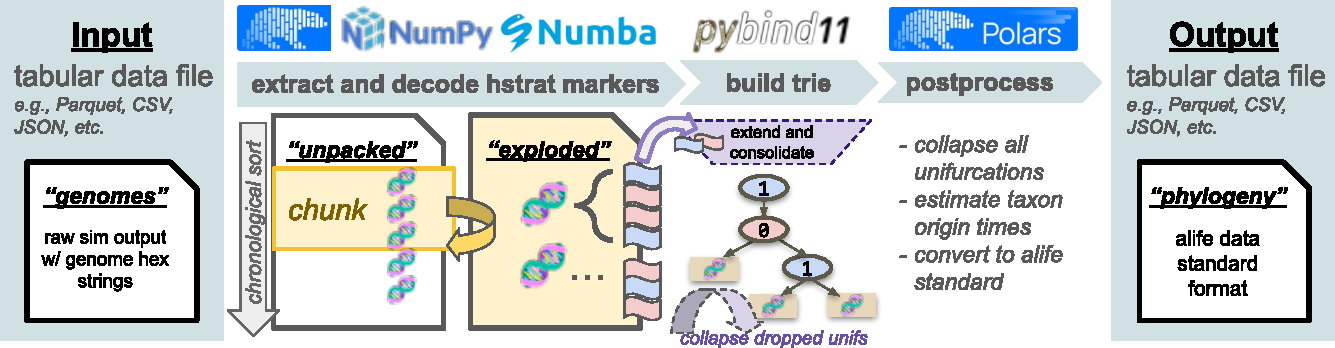
\includegraphics[width=\linewidth]{img/hstratpipeline.pdf}
\caption{\textbf{Schematic of hstrat phylogeny reconstruction pipeline.} TODO.}
\label{fig:hstratpipeline}
\end{figure*}


Figure \ref{fig:hstratpipeline} overviews the full end-to-end pipeline used to construct a phylogeny from raw hstrat-annotated genome data.
First, hstrat annotation data is extracted and decoded.
To take advantage of SIMD parallelism, the decoding of origin times for genome markers is performed using bulk operations orchestrated via NumPy, batched over available processors using the Numba library threading engine.
Due to memory-intensity of the exploded representation, where each genome marker constitutes an individual dataframe row, a chunk size may be configured to limit the amount of data exploded at any one time.
A chunk size of 50 million genomes was used for macrobenchmark trials.

Subsequently, decoded marker data is fed batchwise into the trie-building backend.
To ensure full hardware utilization, execution of the core trie-building procedure -- which is single-threaded -- is overlapped with decode/explode work on the upcoming chunk through multiprocessing.
Finally, a phylogeny is extracted from the final trie, converted to alife standard format, and saved to disk.
The Polars library is used for load/save and other pre-/post-processing operations, allowing some operations to be distributed over available processor cores by the underlying threading engine.

\subsection{Software and Data Availability} \label{sec:materials}

Software used in this work is available via GitHub\footnote{The benchmarking and validation code is available at \href{https://github.com/anony4review/hstrat-reconstruction-algo}{\texttt{anony4review/hstrat-reconstruction-algo}}, WSE kernel code at \href{https://github.com/anony4review/wse-async-ga}{\texttt{anony4review/wse-async-ga}}, and hstrat library code at \href{https://github.com/anony4review/hstrat}{\texttt{anony4review/hstrat}}}.
Data and supplementary material is hosted via the Open Science Framework at \href{https://osf.io/63ucz/?view_only=2e3ec335c016436494ad125b14ffc8cb}{\texttt{osf.io/63ucz}} \citep{supplemental,foster2017open}.
All accompanying materials are provided open-source under the MIT License.

This project benefited significantly from open-source scientific software \citep{2020SciPy-NMeth,harris2020array,reback2020pandas,mckinney2010data,waskom2021seaborn,hunter2007matplotlib,moreno2023teeplot,moreno2024downstream}.